\documentclass[12pt,a4paper]{report}
\usepackage[utf8]{inputenc}
\usepackage{amsmath}
\usepackage{amsfonts}
\usepackage{amssymb}
\usepackage{graphicx}
\usepackage{float}
\usepackage[utf8]{inputenc}
\usepackage[left=2cm,right=2cm,top=2cm,bottom=2cm]{geometry}
\renewcommand{\thesection}{\arabic{section}}
\author{Braydan Newman - n11272031}
\title{Deployment of Network Security Controls}

\begin{document}
\maketitle
\tableofcontents

\newpage

\section{Vulnerability Management}
\subsection{Introduction to Vulnerability Scanning and Prioritisation}
Vulnerability scanning is used to automatically identify weaknesses in an organization's systems, networks, or applications by detecting outdated software, misconfigurations, or known vulnerabilities. The purpose is to provide a clear overview of potential security risks that could be exploited by attackers, enabling timely fixes.

Vulnerability prioritisation is crucial because not all vulnerabilities pose the same level of threat. By ranking them based on severity, impact, and likelihood of exploitation, organizations can focus on addressing the most critical issues first, ensuring that resources are used effectively to mitigate high-risk vulnerabilities.

In the broader scope of network security, vulnerability scanning and prioritisation are essential components of proactive defense. They complement other security measures like firewalls, intrusion detection, and patch management by continuously assessing and addressing risks, helping to maintain a resilient security posture over time.

\subsection{Role of NVD in Vulnerability Scanning and Prioritisation}
The National Vulnerability Database (NVD) is a comprehensive repository of publicly disclosed cybersecurity vulnerabilities, maintained by the U.S. National Institute of Standards and Technology (NIST). It provides standardized data, including severity scores (using CVSS), descriptions, and impact ratings for vulnerabilities. The NVD is significant in vulnerability management because it helps organizations identify and assess vulnerabilities in their systems by referencing a trusted, centralized source. It also supports automation by integrating with various security tools, enabling more efficient vulnerability detection and prioritization efforts.

\subsection{Identification, Assessment and Prioritisation of Vulnerable Services}

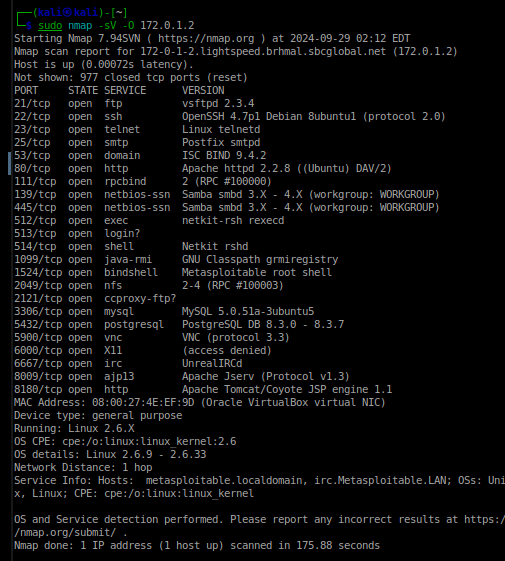
\includegraphics[scale=1]{remmina_lab-71b59751-cf7c-46af-9c75-5b732ca5c73e.australiaeast.cloudapp.azure.com_7095_lab-71b59751-cf7c-46af-9c75-5b732ca5c73e.australiaeast.cloudapp.azure.com_7095_20240929-062627.png} 

\newpage

\begin{table}[h]
\centering
\resizebox{\columnwidth}{!}{%
\begin{tabular}{|l|l|l|l|l|l|l|}
\hline
\begin{tabular}[c]{@{}l@{}}Vulnerable \\ service\end{tabular} &
  \begin{tabular}[c]{@{}l@{}}Vulnerability ID \\ and CWE ID\end{tabular} &
  Short description &
  Severity (CVSS) &
  \begin{tabular}[c]{@{}l@{}}Associated Vector \\ (metrics) here provide\end{tabular} &
  \begin{tabular}[c]{@{}l@{}}Affected \\ Product\end{tabular} &
  Remediation action \\ \hline
vsftpd &
  \begin{tabular}[c]{@{}l@{}}CVE-2011-2523\\ CWE-78\end{tabular} &
  \begin{tabular}[c]{@{}l@{}}Contains a backdoor which \\ can open a shell on port 6200/tcp\end{tabular} &
  9.8 CRITICAL &
  \begin{tabular}[c]{@{}l@{}}Network, \\ Low complexity\end{tabular} &
  Vsftpd &
  \begin{tabular}[c]{@{}l@{}}Update software to \\ version above 20110703\end{tabular} \\ \hline
ISC BIND &
  \begin{tabular}[c]{@{}l@{}}CVE-2008-0122\\ CWE-189\end{tabular} &
  \begin{tabular}[c]{@{}l@{}}An off-by-one error that can \\ allow for DOS and ACE\end{tabular} &
  10.0 HIGH &
  \begin{tabular}[c]{@{}l@{}}Network, \\ Low complexity\end{tabular} &
  BIND 9 &
  \begin{tabular}[c]{@{}l@{}}Patch Software to version \\ 7.0-PRERELEASE, \\ or 6-STABLE\end{tabular} \\ \hline
Linux kernel &
  \begin{tabular}[c]{@{}l@{}}CVE-2007-6762\\ CWE-119\end{tabular} &
  \begin{tabular}[c]{@{}l@{}}\textbackslash{}An off-by-one error that \\ can allow for DOS and ACE\end{tabular} &
  9.8 CRITICAL &
  \begin{tabular}[c]{@{}l@{}}Network, \\ Low complexity\end{tabular} &
  Linux &
  \begin{tabular}[c]{@{}l@{}}Apply patching git commit \\ 2a2f11c227bdf292b3a\\ 2900ad04139d301b56ac4\end{tabular} \\ \hline
MySQL &
  \begin{tabular}[c]{@{}l@{}}CVE-2009-4484\\ CWE-787\end{tabular} &
  \begin{tabular}[c]{@{}l@{}}Multiple buffer overflow \\ vulnerability’s that allows for DOS \\ and ACE\end{tabular} &
  7.5 HIGH &
  Network, N/A &
  MySQL &
  \begin{tabular}[c]{@{}l@{}}Update to latest \\ version of MySQL\end{tabular} \\ \hline
PostgreSQL &
  \begin{tabular}[c]{@{}l@{}}CVE-2009-0922\\ CWE-399\end{tabular} &
  \begin{tabular}[c]{@{}l@{}}By triggering a failure in the \\ conversion of a localized error message \\ one allows remote authenticated users \\ to cause a denial of service\end{tabular} &
  4.0 MEDIUM &
  \begin{tabular}[c]{@{}l@{}}Network, \\ Low complexity\end{tabular} &
  PostgreSQL &
  \begin{tabular}[c]{@{}l@{}}Patch PostgreSQL to version \\ 8.3.7, 8.2.13, 8.1.17, 8.0.21, \\ or 7.4.25\end{tabular} \\ \hline
\end{tabular}%
}
\end{table}

\subsection{Complementary Controls for Vulnerability Scanning and Prioritisation}

A complementary control for vulnerability scanning and prioritisation is penetration testing, where security professionals simulate real-world attacks to actively exploit vulnerabilities in a system. Unlike automated vulnerability scans, penetration testing provides deeper insight by assessing how vulnerabilities can be exploited in practice, identifying risks that might be missed or misclassified by scanning tools. This hands-on approach allows organizations to better understand the potential impact of vulnerabilities and helps prioritize fixes based on real-world exploitability, enhancing the overall risk assessment process.

\section{Intrusion Detection System}
\subsection{Introduction to Intrusion Detection System - Snort}

An Intrusion Detection System (IDS) monitors network traffic to detect suspicious activities or potential security threats, alerting administrators when unusual behavior is detected. Its primary role is to identify potential breaches and malicious activities in real-time to maintain network security.

Snort, a popular open-source IDS, functions by analyzing network traffic against predefined rules to identify known attack patterns. It features packet sniffing, protocol analysis, and real-time intrusion detection capabilities, enabling administrators to detect and respond to threats effectively.

\subsection{Different ways to use or deploy Snort}
\paragraph{Deployment methods for Snort}

\begin{description}
   \item[Network Intrusion Detection System (NIDS)] In this mode, Snort inspects network traffic passively and generates alerts when it detects suspicious activities or signatures that match its rule set. It doesn't block or modify the traffic, making it ideal for monitoring.
   
   \textit{snort.conf}
   \begin{verbatim}
# Specify network variables
var HOME_NET 192.168.1.0/24
var EXTERNAL_NET any

# Define the rule files
include $RULE_PATH/local.rules
include $RULE_PATH/community.rules

# Enable logging and alerting
output alert_fast: /var/log/snort/alerts.log
output unified2: filename snort.u2, limit 128

# Preprocessors for detecting various attack types
preprocessor stream5_global: track_tcp yes, track_udp yes, track_icmp no
preprocessor stream5_tcp: policy windows, detect_anomalies
preprocessor http_inspect: global iis_unicode_map unicode.map 1252

	\end{verbatim}
   
   
	\item[Intrusion Prevention System (IPS)] In IPS mode, Snort actively blocks or modifies traffic that matches a set of rules. It can drop, reject, or alert on malicious packets to prevent the attack from succeeding.
	
	\textit{local.rules}
	
	\begin{verbatim}
alert tcp any any -> $HOME_NET 80 (msg:"Suspicious Web Traffic";
 flow:to_server,established; content:"malicious"; sid:1000001; rev:1;)
 
drop tcp any any -> $HOME_NET 80 (msg:"Block Malicious Traffic";
 flow:to_server,established; content:"evil_payload"; sid:1000002; rev:1;)

	\end{verbatim}
      
	\item[Packet Logger] Snort can be used in packet logger mode to log all network traffic that passes through a specific network interface. This is useful for network forensics or deep packet inspection.
	
	\textit{snort.conf}
	
	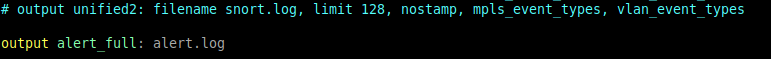
\includegraphics[scale=.5]{remmina_lab-71b59751-cf7c-46af-9c75-5b732ca5c73e.australiaeast.cloudapp.azure.com_7095_lab-71b59751-cf7c-46af-9c75-5b732ca5c73e.australiaeast.cloudapp.azure.com_7095_20241002-065916.png} 	
\end{description}

\newpage

\textbf{Proof of me doing it}\\

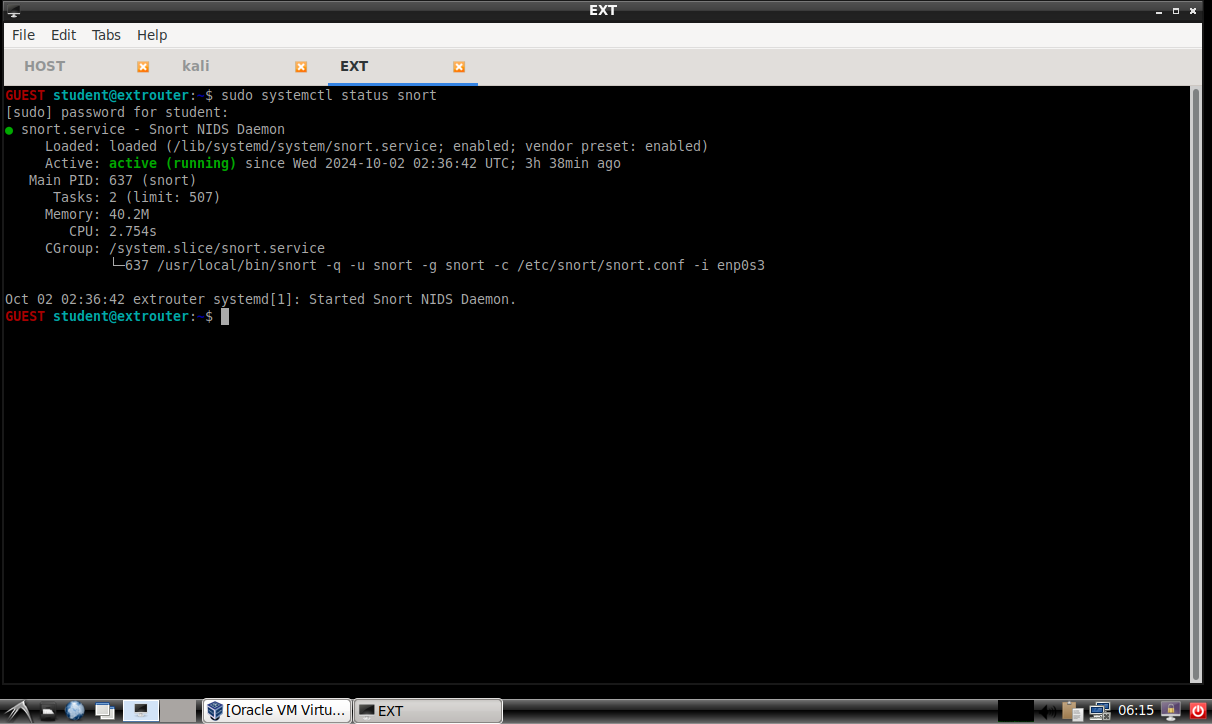
\includegraphics[scale=.25]{snort active.png} \\
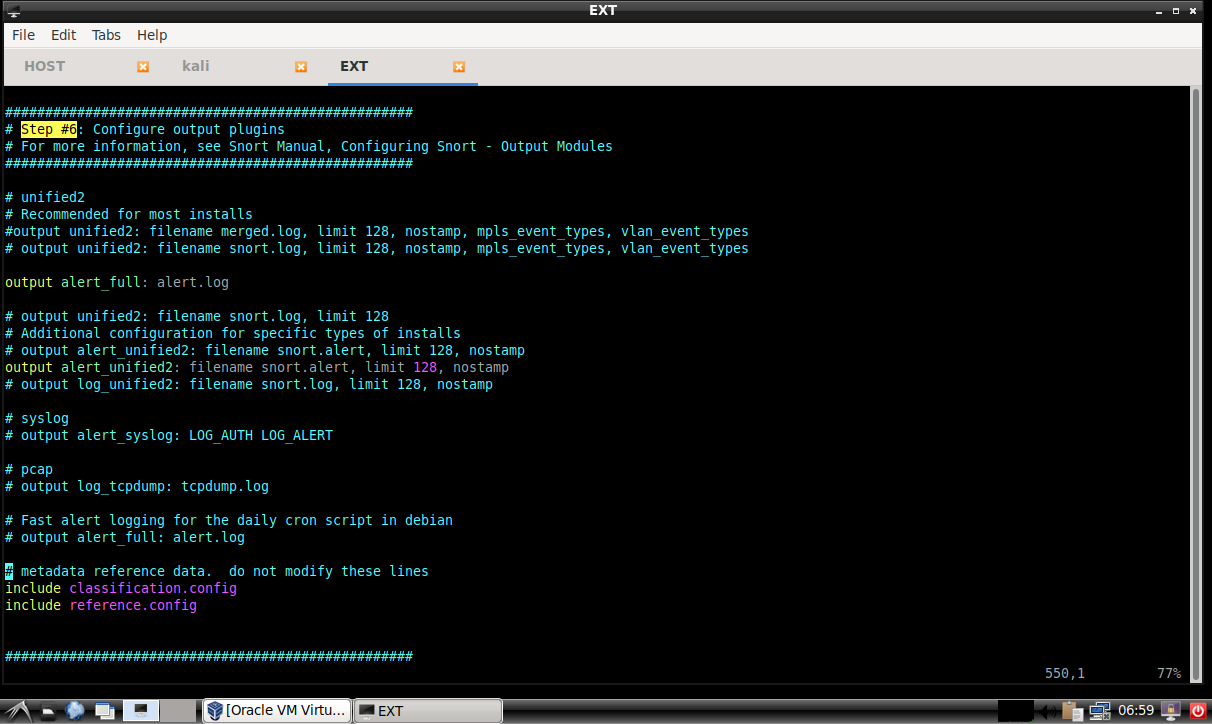
\includegraphics[scale=.25]{snort config.png} \\
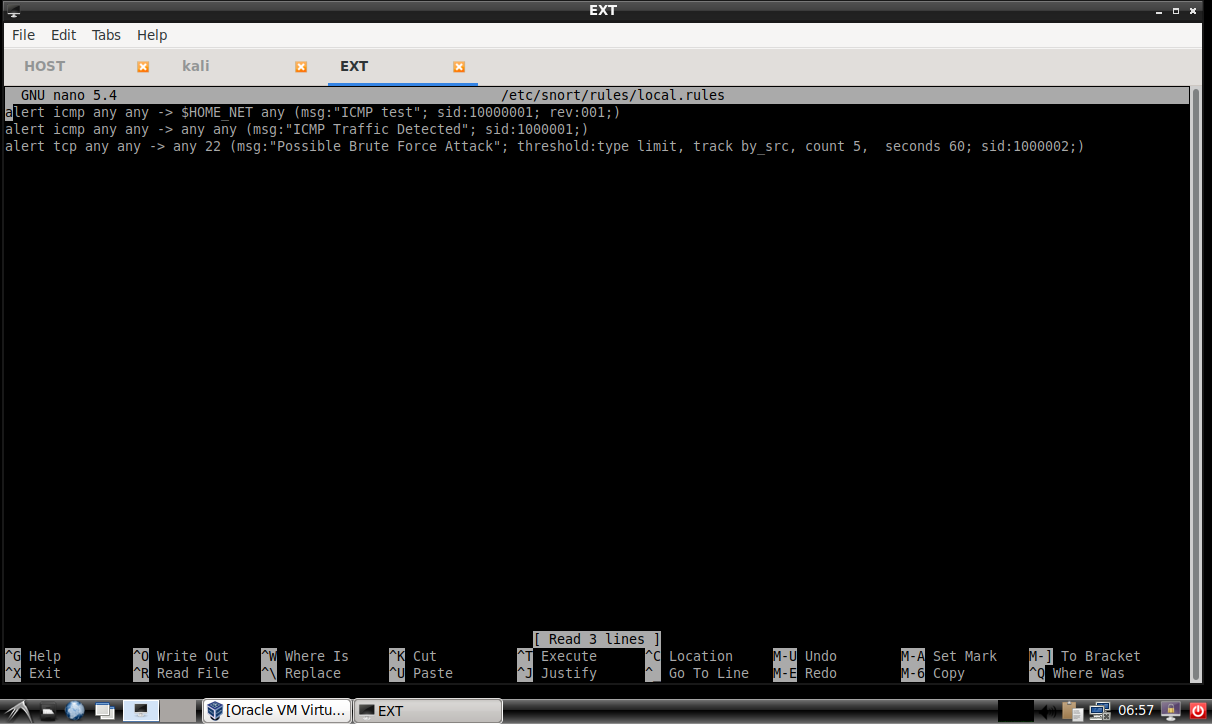
\includegraphics[scale=.25]{rule config.png} \\

\newpage





\subsection{Logging and Monitoring Snort Alerts}

\begin{description}
   \item[Fast Alert Mode (Fast Logging)] Fast Alert Mode is a simplified logging method where alerts are written in a concise, human-readable format. It provides only essential information about each alert, making it ideal for quick scanning and troubleshooting.
   
	\item[Unified2 Format (Binary Logging for Centralized Monitoring)] The Unified2 format is a binary logging method suitable for use with centralized alert collection and analysis systems like Snorby, Barnyard2, or Security Onion. It captures more detailed data than the fast alert mode, making it ideal for large-scale or production environments.
      
	\item[Syslog (Remote Logging and Integration with SIEM Systems)] Snort can send alerts directly to a syslog server, which can then forward these logs to a centralized monitoring system such as a Security Information and Event Management (SIEM) system (e.g., Splunk, Graylog, or ELK Stack). This method is ideal for real-time alerting and centralized monitoring.
	
\end{description}

\textbf{The three different ways to log and monitor Snort Alerts}\\
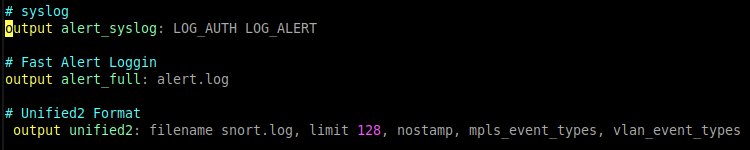
\includegraphics[scale=0.6]{loging stuff.png} 

\subsection{Detecting Risks and Attacks using Snort}

This will consist of 3 attacks:
\begin{enumerate}
  \item Brute Force Attack on SSH
  \item ICMP (Ping) Flood (Denial of Service Attack)
  \item Port Scanning (nmap) detection, which is commonly used when attacking a system or network
\end{enumerate}

Here are the snort rule set used for the 3 attacks.

\begin{figure}[H]
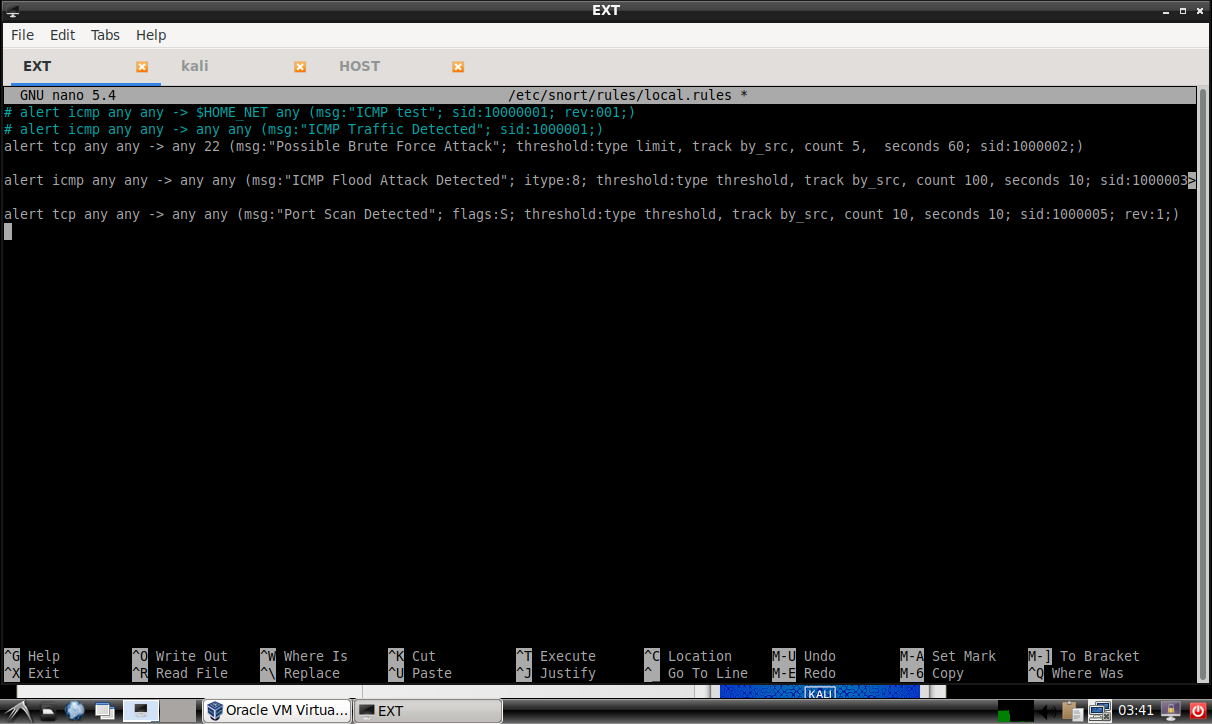
\includegraphics[scale=.3]{rule config 2.png} 
\end{figure}

\begin{description}
	\item[Brute Force Attack on SSH] A brute force attack involves trying multiple combinations of usernames and passwords in an attempt to gain unauthorized access to a service, like SSH. The attacker typically uses tools like Hydra or Medusa to automate the guessing process. Snort can detect such attacks by identifying multiple failed login attempts from the same IP address.
	
\begin{figure}[H]
    \centering
    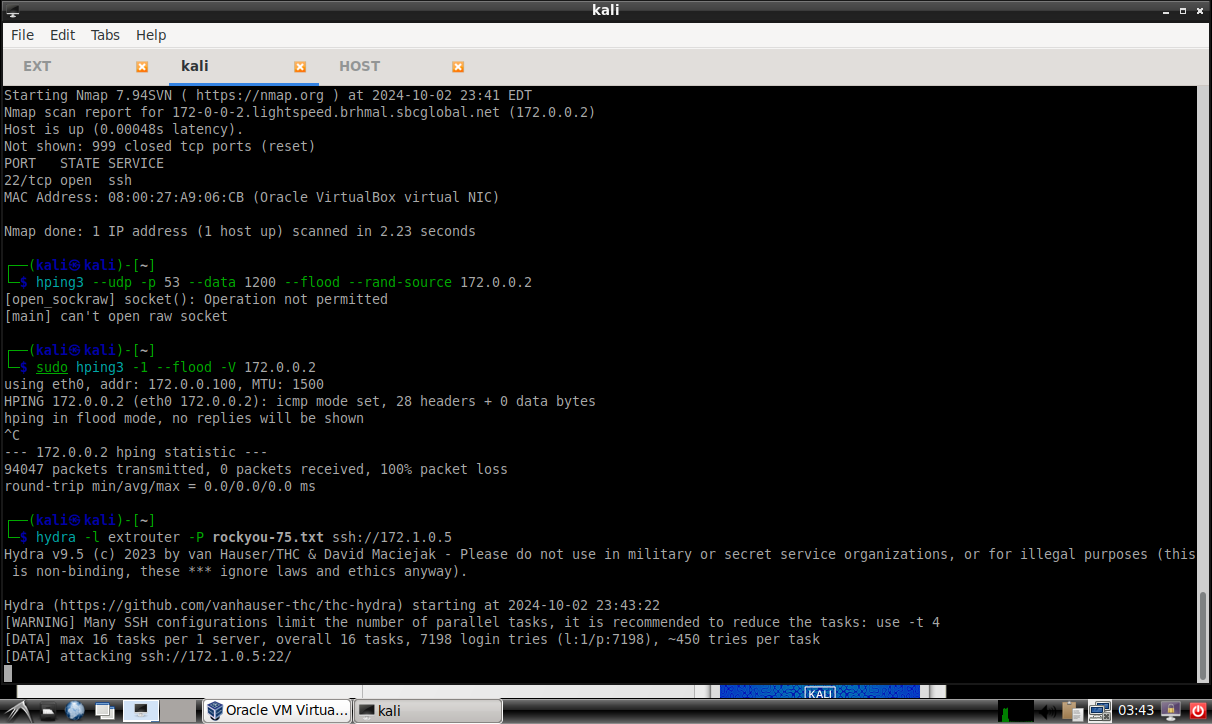
\includegraphics[width=\textwidth]{ssh attk.png} 
    \caption{Screenshot showing an SSH Attack in progress using the hydra tool}
    \label{fig:mesh1}
\end{figure}

\begin{figure}[H]
    \centering
    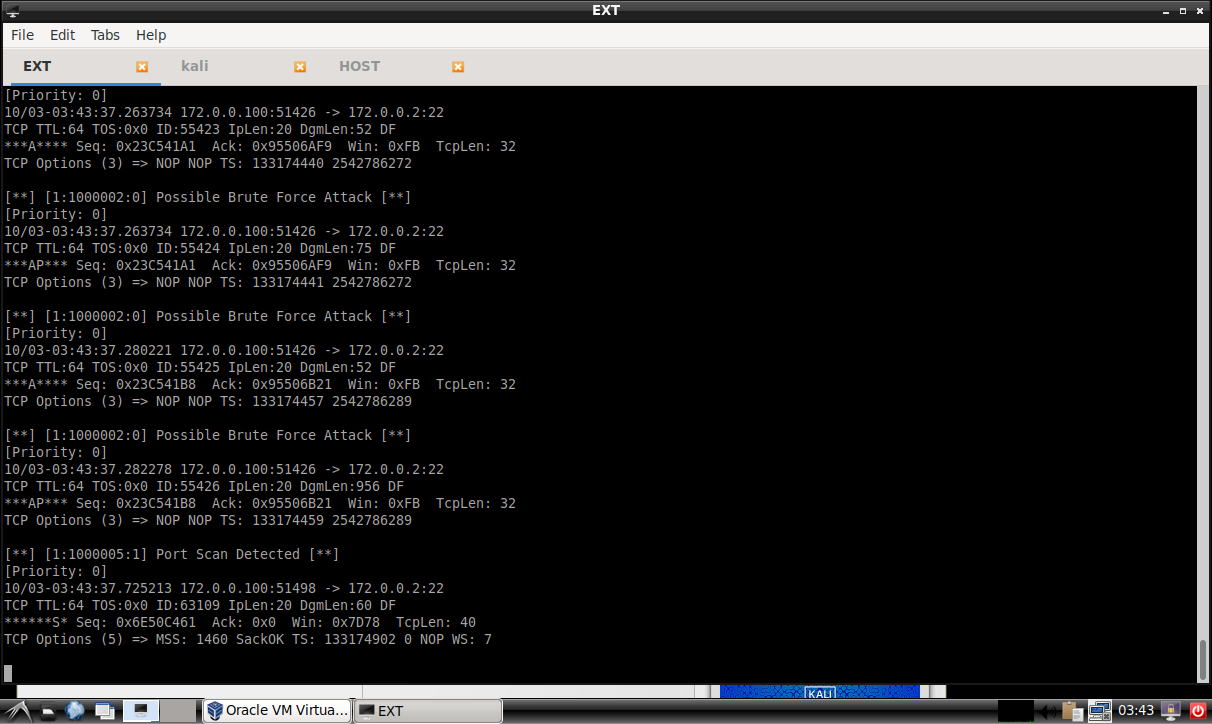
\includegraphics[width=\textwidth]{ssh logs.png} 
    \caption{Screenshot showing Snort alerts about a SSH Attack }
    \label{fig:mesh1}
\end{figure}
	
   
	\item[ICMP (Ping) Flood (Denial of Service Attack)] A Ping Flood or ICMP flood attack involves sending a large number of ICMP echo request (ping) packets to a target system, overwhelming it and potentially causing a Denial of Service (DoS). Snort can detect this attack by monitoring the rate of ICMP requests coming from the same source IP.
	
\begin{figure}[H]
    \centering
    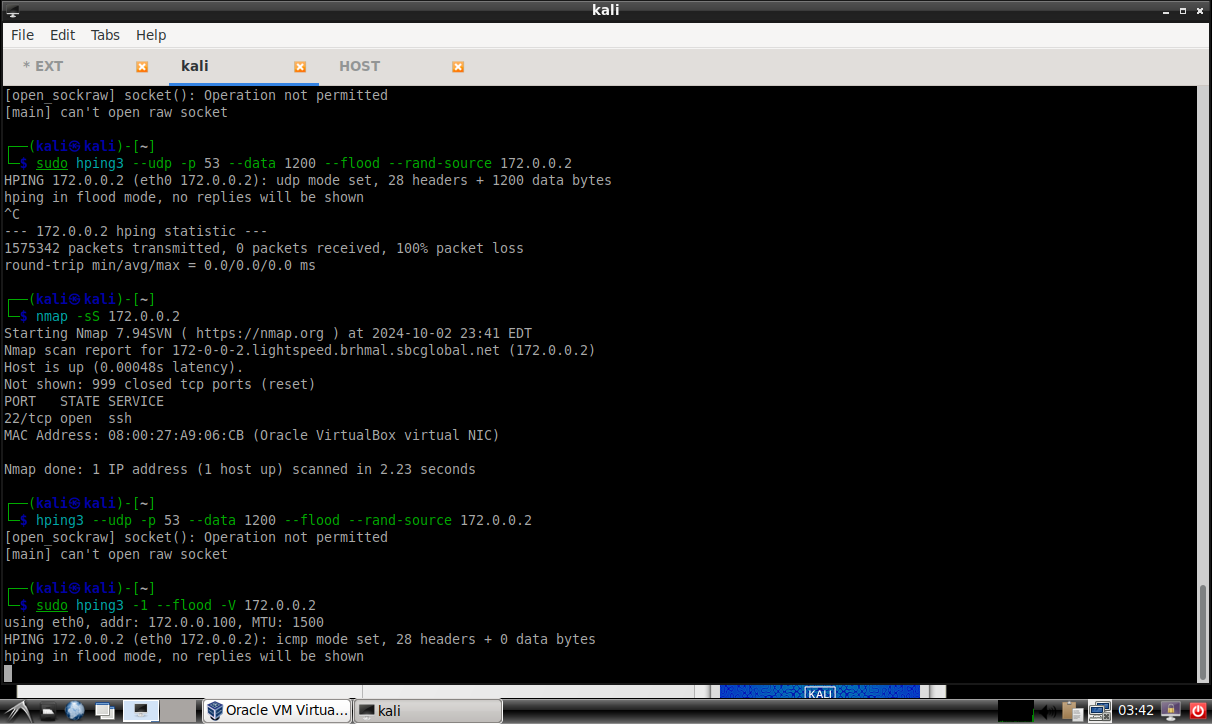
\includegraphics[width=\textwidth]{flood attk.png} 
    \caption{Screenshot showing an ICMP in progress using the hping3 tool}
    \label{fig:mesh1}
\end{figure}

\begin{figure}[H]
    \centering
    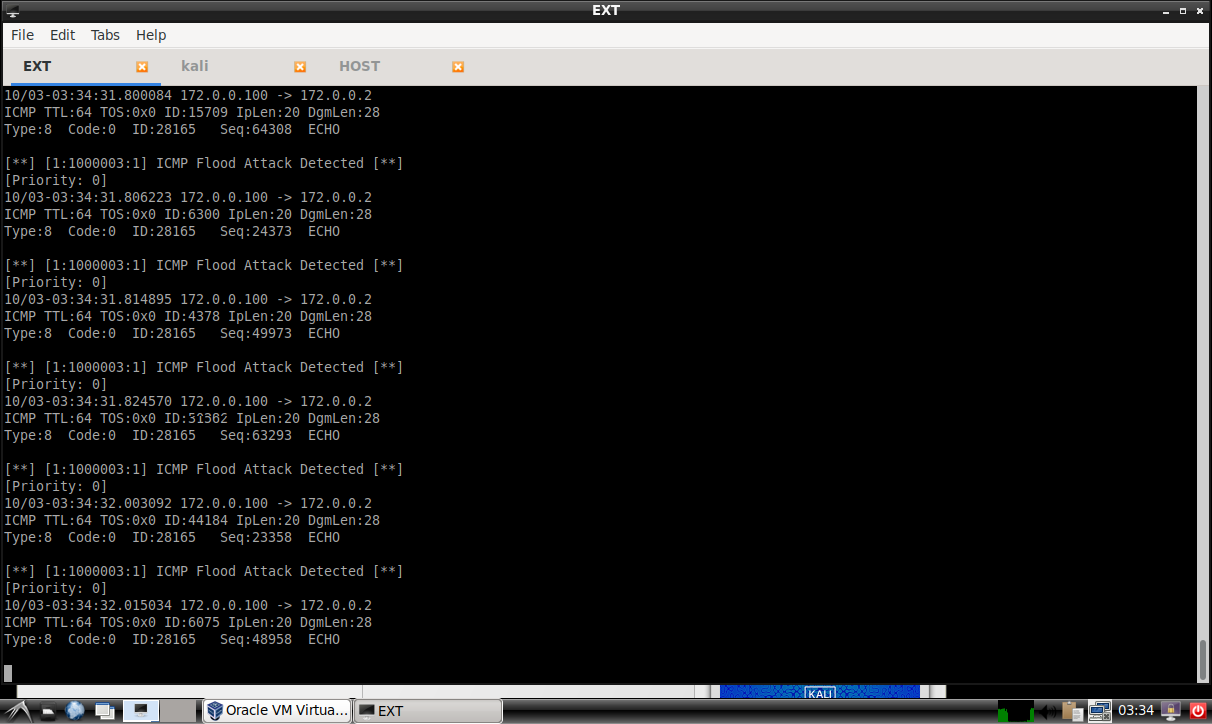
\includegraphics[width=\textwidth]{flood logs.png} 
    \caption{Screenshot showing Snort alerts about a ICMP Flood Attack}
    \label{fig:mesh1}
\end{figure}
	
	
      
	\item[Port Scanning (Nmap)] Port scanning is often used by attackers to identify open ports and services on a target system. Tools like Nmap are commonly used for this purpose. While port scanning isn't inherently malicious, it is often a precursor to more serious attacks. Snort can detect port scanning by monitoring for multiple connection attempts to different ports from the same source IP.
	
\begin{figure}[H]
    \centering
    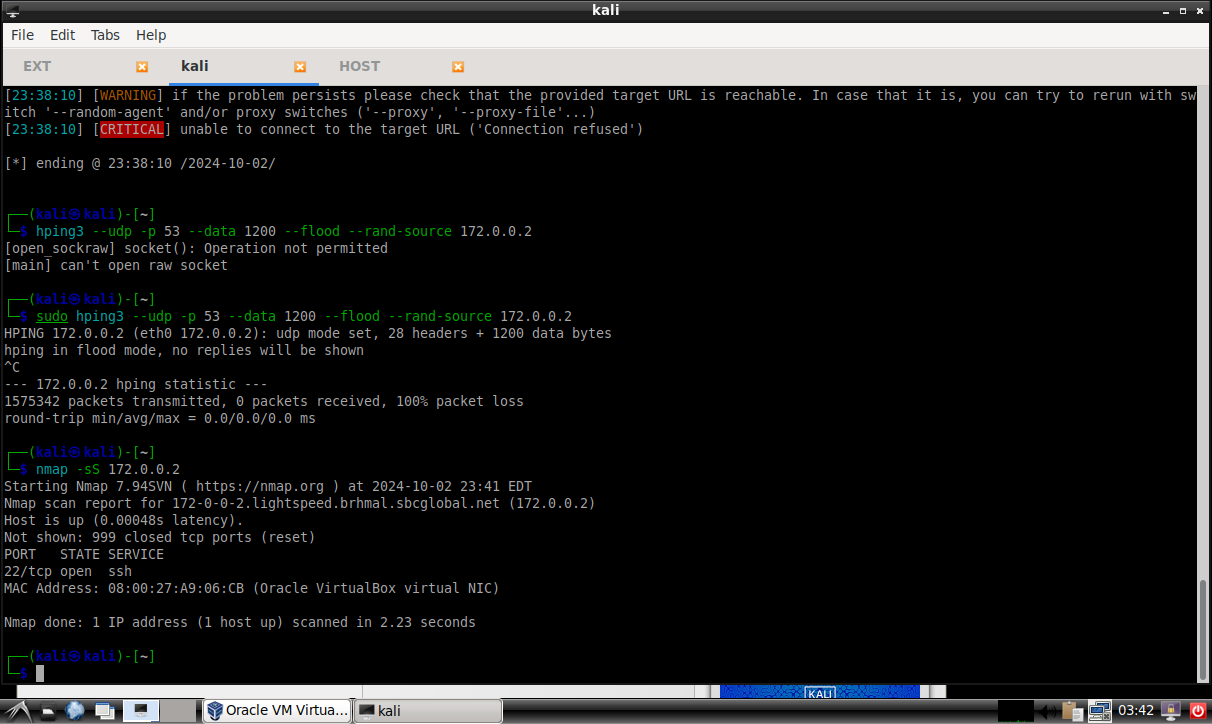
\includegraphics[width=\textwidth]{port scan attk.png} 
    \caption{Screenshot showing an Port Scan in progress using the NMAP tool}
    \label{fig:mesh1}
\end{figure}

\begin{figure}[H]
    \centering
    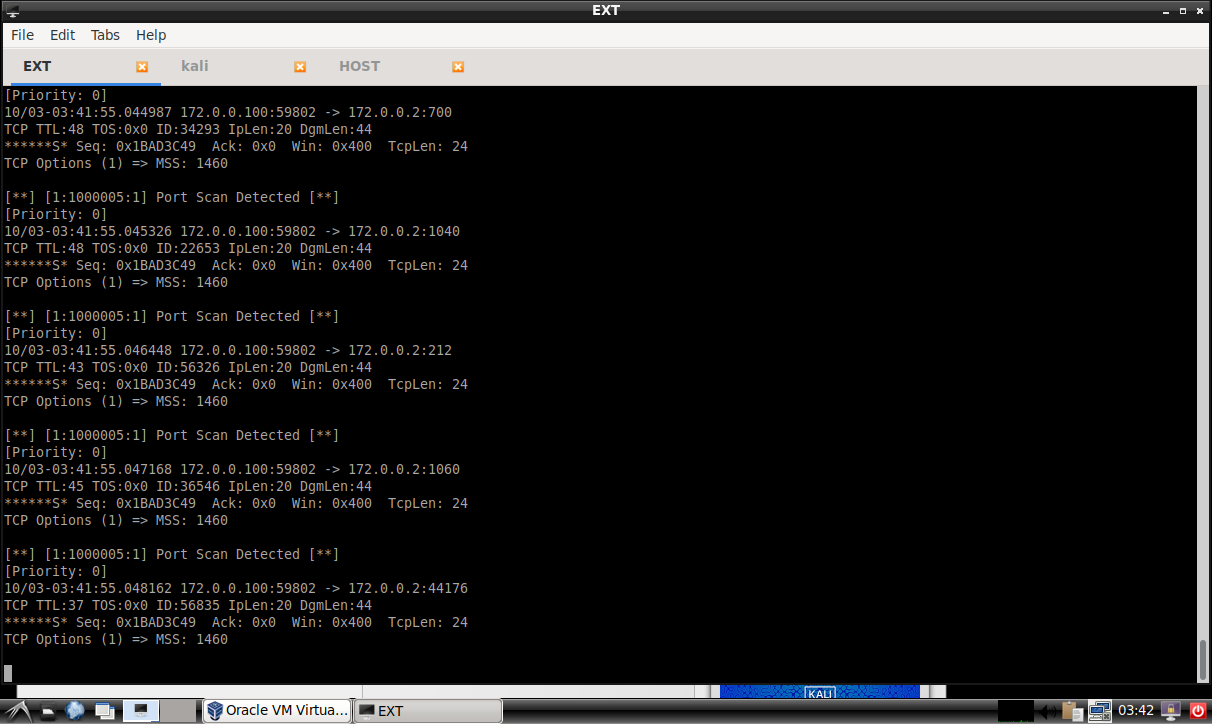
\includegraphics[width=\textwidth]{port scan logs.png} 
    \caption{Screenshot showing Snort alerts about a Port Scan}
    \label{fig:mesh1}
\end{figure}

\end{description}

\newpage

\subsection{Complementary Controls for IDS}

\begin{description}
	\item[Firewall with Intrusion Prevention Capabilities (WAF or Network-Based Firewall)] A firewall with built-in Intrusion Prevention System (IPS) or Web Application Firewall (WAF) capabilities can provide an additional layer of protection against various types of attacks, including SQL Injection (SQLi), Cross-Site Scripting (XSS), and Brute Force Attacks.
	
	
	\item[Network Segmentation and Access Control Lists (ACLs)] Network Segmentation involves dividing a network into smaller sub-networks (or segments) to restrict lateral movement of attackers and limit access to critical systems. Combined with Access Control Lists (ACLs), this control helps mitigate risks from Port Scanning, DNS Amplification Attacks, and other reconnaissance activities by limiting access to sensitive services or devices.
	
\end{description}


\section{Proxies}
\subsection{Main purposes of Proxy}

\begin{description}
	\item[Adding TLS to a Web Server Using a Reverse Proxy] In this setup, a reverse proxy is used to add TLS encryption to a web server. The reverse proxy terminates TLS (HTTPS) connections from clients and forwards requests to the backend web server, which may not support TLS itself.


\textbf{Security Goals:}
\begin{description}
	\item[Confidentiality] LS encrypts the communication between the client and the reverse proxy, ensuring sensitive information (e.g., login credentials, personal data) isn’t intercepted by attackers during transmission.
	\item[Integrity] TLS also protects against data tampering during transmission. If data is modified in transit, the client or server will detect it through cryptographic checks.
	\item [Availability] Reverse proxies can distribute traffic across multiple backend servers, preventing one server from being overwhelmed. This improves uptime and availability.
\end{description}


\textbf{Security Principles:}
\begin{description}
	\item[Defense in Depth] The reverse proxy acts as an additional layer of security between the client and the backend server, reducing direct exposure of the internal server.
	\item[ISeparation of Responsibilities] The proxy manages TLS encryption, offloading the complexity from the backend server. This ensures a more manageable security architecture.
	\item[Fail-Safe Defaults] If the TLS handshake fails or the proxy server detects suspicious behavior, connections can be rejected, reducing risks from improperly configured or malicious requests.
\end{description}

	
	
	\item[Setting up a Web Proxy with Filtering] This configuration involves using mitmproxy to intercept, inspect, and filter HTTP/HTTPS traffic between clients and servers. The proxy sits between the client and the target website, decrypting and analyzing the content before passing it along.
	
	\textbf{Security Goals:}
\begin{description}
	\item[Confidentiality] Although mitmproxy intercepts encrypted traffic, in legitimate scenarios (such as internal monitoring), it helps ensure that only authorized users or systems can view sensitive data.
	\item[Integrity] mitmproxy allows filtering to block or modify malicious traffic, ensuring only legitimate and safe data reaches clients or servers.
	\item [Availability] By blocking harmful or unnecessary traffic (e.g., ads, malicious scripts), mitmproxy ensures that only important resources are accessed, optimizing network availability and reducing strain.
\end{description}


\textbf{Security Principles:}
\begin{description}
	\item[Least Privilege] Mitmproxy can be configured to monitor or filter only specific traffic types, ensuring that the proxy doesn’t access more data than necessary.
	\item[Inspection and Auditing] The proxy can be used to log and inspect traffic, supporting security audits and monitoring for compliance or security policy violations.
	\item[Fail-Secure Stance] If mitmproxy detects malicious behavior or harmful content, it can block connections, preventing compromised data from reaching the client or server.
\end{description}
\end{description}

\begin{figure}[H]
    \centering
    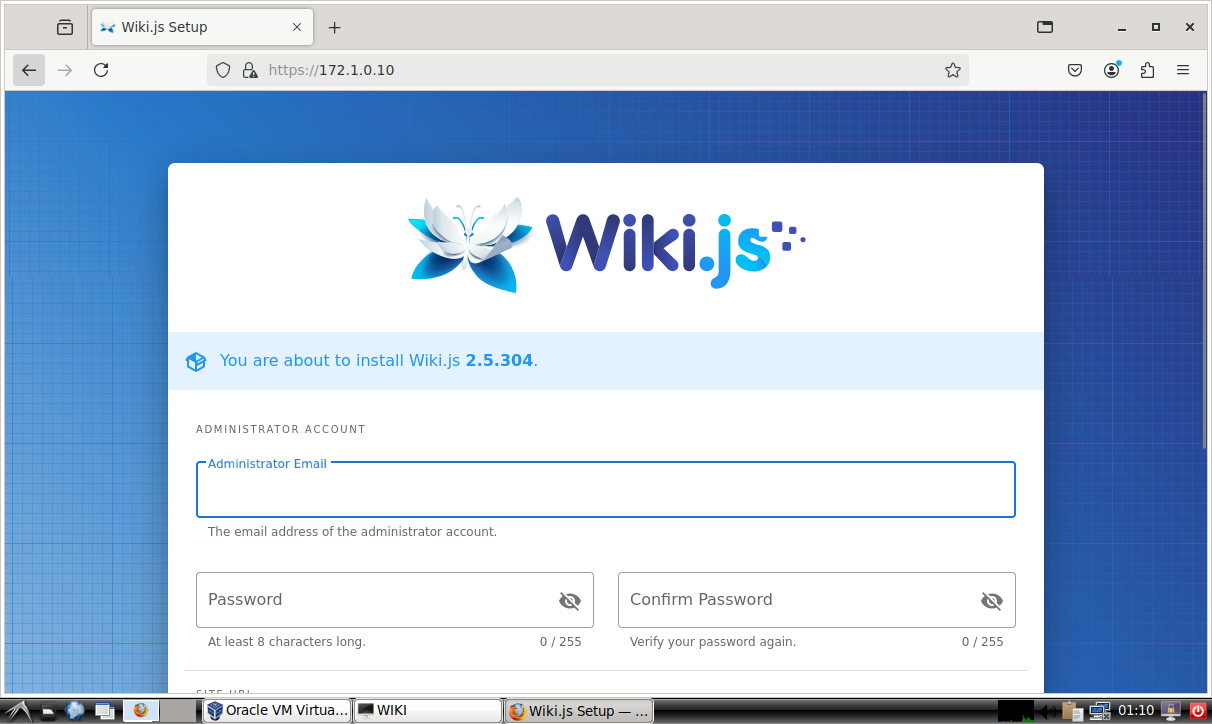
\includegraphics[width=\textwidth]{nginx proxy url and web page.png} 
    \caption{Web Page and URL of the nginx Proxy}
    \label{fig:mesh1}
\end{figure}

\begin{figure}[H]
	\centering
	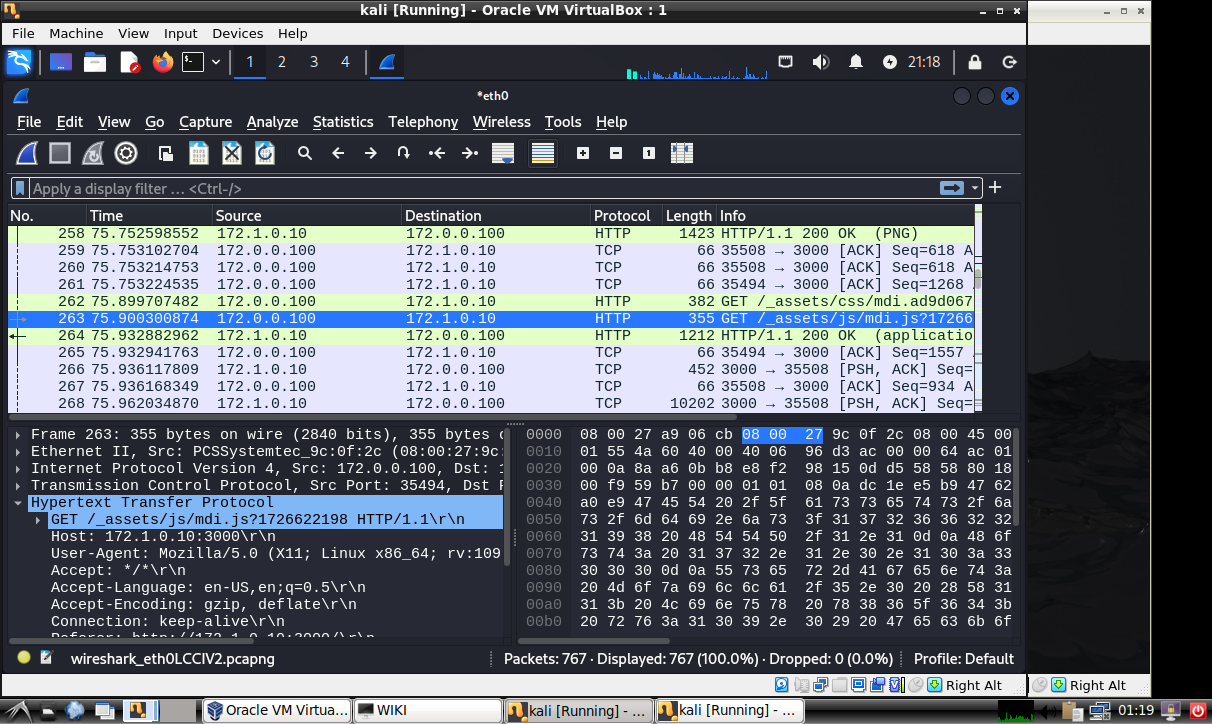
\includegraphics[width=\textwidth]{wireshark unencrypted packet captures.png}
	\caption{Wireshark unencrypted packet capture}
\end{figure}

\begin{figure}[H]
	\centering
	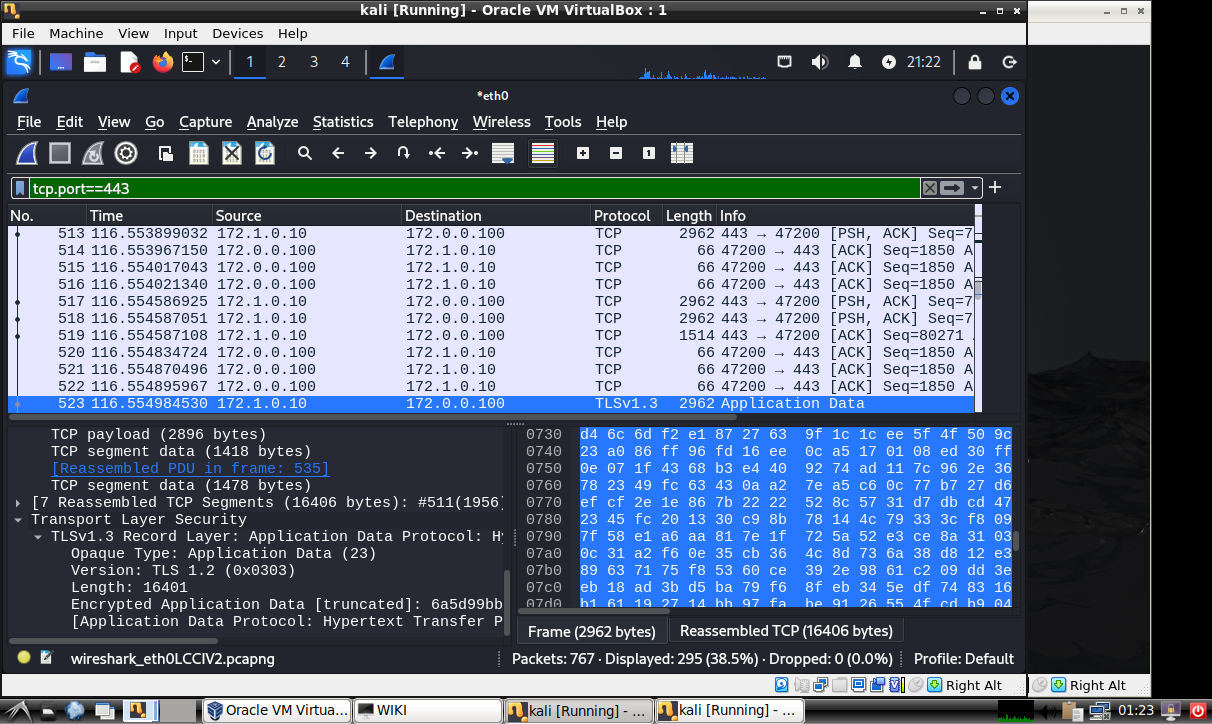
\includegraphics[width=\textwidth]{wireshark encrypted packet captures.png}
	\caption{Wireshark encrypted packet capture}
\end{figure}

\textbf{MISSING SCREENSHOTS - No Internet connection on Kali VM: }

\begin{itemize}
\item Set up Firefox on Kali to use the proxy
\item Configure some filtering
\end{itemize}


\subsection{Remaining Risk}
Risks associated with each proxy configuration:\\

\textbf{Adding TLS to a Web Server Using a Reverse Proxy}
\begin{enumerate}
	\item \textbf{TLS Misconfiguration Risk} - If the TLS configuration (e.g., cipher suites, certificates, or protocols) is not properly managed, the proxy might allow weak encryption methods, making it vulnerable to attacks such as downgrade attacks or cipher vulnerabilities (e.g., SWEET32). This can compromise the confidentiality and integrity of data in transit.
	
	\item \textbf{Man-in-the-Middle Attack on the Proxy} - While the reverse proxy secures connections between the client and the proxy, attackers could target the connection between the reverse proxy and backend server if it isn't secured properly. This risk exposes backend data to interception or tampering.
	
	\item \textbf{Single Point of Failure} - If the reverse proxy fails, the entire system may become unavailable. Although proxies often support high availability through load balancing, misconfigured failover mechanisms could still result in downtime and affect availability.
\end{enumerate}

\textbf{Setting up a Web Proxy with Filtering Using mitmproxy}
\begin{enumerate}
	\item \textbf{Privacy and Ethical Risks} - Since mitmproxy decrypts and inspects encrypted traffic, it can capture sensitive information such as passwords or personal data. This introduces privacy risks if access to logs or captured data is not properly controlled, or if the system is used unethically.
	
	\item \textbf{Potential Introduction of New Vulnerabilities} - Intercepting and re-encrypting traffic introduces another point of vulnerability. If the proxy mishandles encryption keys or fails to re-encrypt traffic correctly, attackers could exploit these weaknesses, compromising the data’s confidentiality and integrity.
	
	\item \textbf{Detection and Evasion by Attackers} - Some sophisticated attackers or malware may detect the presence of a proxy and attempt to bypass it by using non-standard protocols, encrypted tunnels, or domain fronting techniques. This can limit the effectiveness of the filtering, leaving the system exposed to threats.
\end{enumerate}

\subsection{Complementary Controls to Proxy}
Complementary controls to mitigate the identified risks: \\

\textbf{Adding TLS to a Web Server Using a Reverse Proxy}
\begin{enumerate}
	\item \textbf{TLS Misconfiguration Risk → Regular Security Audits and Hardened Configuration} - Conduct periodic audits of the TLS configuration using tools like SSL Labs or OpenSSL to identify weak cipher suites and protocols. Implement hardened TLS settings (e.g., disabling TLS 1.0/1.1, using strong ciphers, and certificate pinning) to mitigate downgrade attacks.
	
	\item \textbf{Man-in-the-Middle Attack on the Proxy → Secure Backend Communication with TLS} - Use TLS encryption between the reverse proxy and backend servers to prevent interception or tampering of internal traffic. Enable mutual TLS (mTLS) authentication between the proxy and backend to ensure that only authorized servers can communicate.
	
	\item \textbf{Single Point of Failure → Load Balancing and Redundancy} - Implement load balancers and configure multiple reverse proxies to distribute traffic evenly. Use health checks and failover mechanisms to ensure availability in case one proxy instance goes down.
\end{enumerate}


\textbf{Setting up a Web Proxy with Filtering Using mitmproxy}
\begin{enumerate}
	\item \textbf{Privacy and Ethical Risks → Access Control and Data Retention Policies} - Implement strict access control to ensure that only authorized personnel can view decrypted traffic or logs. Establish data retention policies that limit how long captured data is stored and ensure sensitive information is deleted promptly.
	
	\item \textbf{Introduction of New Vulnerabilities → Secure Key Management and Patching} - Use a centralized key management system to securely store and rotate encryption keys used by the proxy. Regularly update and patch the proxy software to address vulnerabilities and improve encryption handling.
	
	\item \textbf{Detection and Evasion by Attackers → Deep Packet Inspection and Anomaly Detection} - Integrate deep packet inspection (DPI) tools alongside mitmproxy to detect non-standard protocols or encrypted tunnels used for evasion. Employ intrusion detection systems (IDS) to monitor for anomalous behavior that could indicate an attacker bypassing the proxy.
\end{enumerate}

\section{Security Information and Event Management (SIEM)}

\subsection{Introduction to SIEM}
Primary purposes and roles of SIEM's

\begin{description}
	\item[Centralized Log Collection and Correlation] SIEM aggregates logs and events from various sources, such as firewalls, proxies, servers, and endpoints, into a unified system. It correlates data across these sources to identify patterns that might indicate security incidents or policy violations.
	
	\item[Real-Time Threat Detection and Alerts] SIEM continuously monitors network traffic and system events to detect suspicious activity, such as unauthorized access attempts or malware. It provides real-time alerts to security teams, enabling swift responses to potential threats.
	
	\item[Incident Response and Forensics] SIEM assists in the investigation of security incidents by providing detailed logs and reports that can help identify the scope and impact of an attack. It supports post-incident analysis and forensics to understand the root cause and improve defenses.
\end{description}

\subsection{Wazuh as SIEM}

Wazuh is an open-source SIEM platform that provides comprehensive security monitoring, threat detection, and incident response capabilities. It collects and analyzes logs from various sources, helping organizations identify security threats, ensure compliance, and manage vulnerabilities.

\paragraph{Features Supporting Security Monitoring and Threat Management}

\begin{description}
	\item[Log Collection and Analysis] Wazuh collects logs from multiple systems (e.g., servers, firewalls, and proxies) and analyzes them to detect suspicious behavior. This aligns with activities such as monitoring HTTP/HTTPS traffic and identifying anomalies in proxy logs, similar to what is achieved with mitmproxy in this tutorial.
	
	\item[File Integrity Monitoring (FIM)] Wazuh tracks changes to critical files and directories, alerting administrators of unauthorized modifications. This feature complements backend security in TLS-based reverse proxies, where ensuring the integrity of configuration files is essential for preventing tampering.
	
	\item[Real-Time Threat Detection] Wazuh uses rules to correlate events and trigger alerts when suspicious activity is detected, such as brute-force attacks or malware. This supports filtering and blocking malicious traffic, much like the functionality explored using mitmproxy for web proxy filtering.
	
	\item[Vulnerability Detection and Compliance Management] Wazuh scans systems for vulnerabilities and ensures they meet compliance standards. This feature can complement TLS hardening activities in the tutorial by ensuring that servers are patched and secure, reducing exposure to attacks.
\end{description}

\begin{figure}[H]
\centering
\includegraphics[width=\textwidth]{Wazuh’s Dashboard.png}
\caption{Wazuh’s Dashboard}
\end{figure}

\begin{figure}[H]
\centering
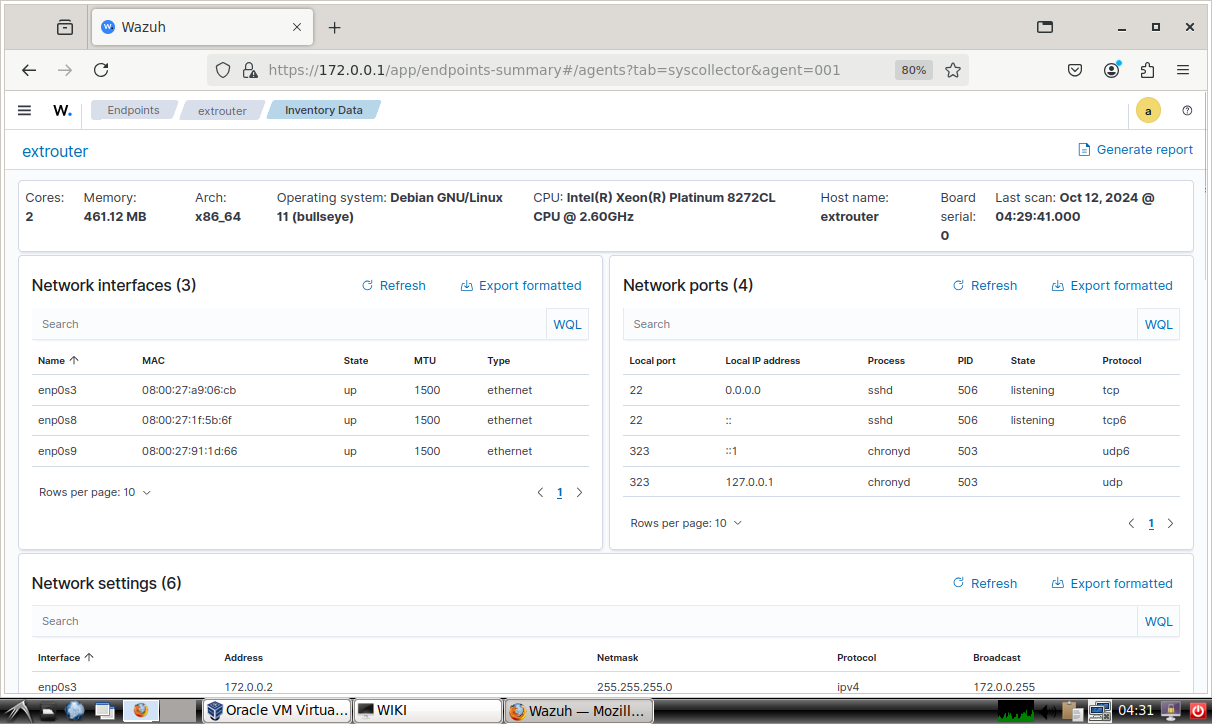
\includegraphics[width=\textwidth]{extrouter details.png}
\caption{Extrouter Wazuh Details}
\end{figure}

\begin{figure}[H]
\centering
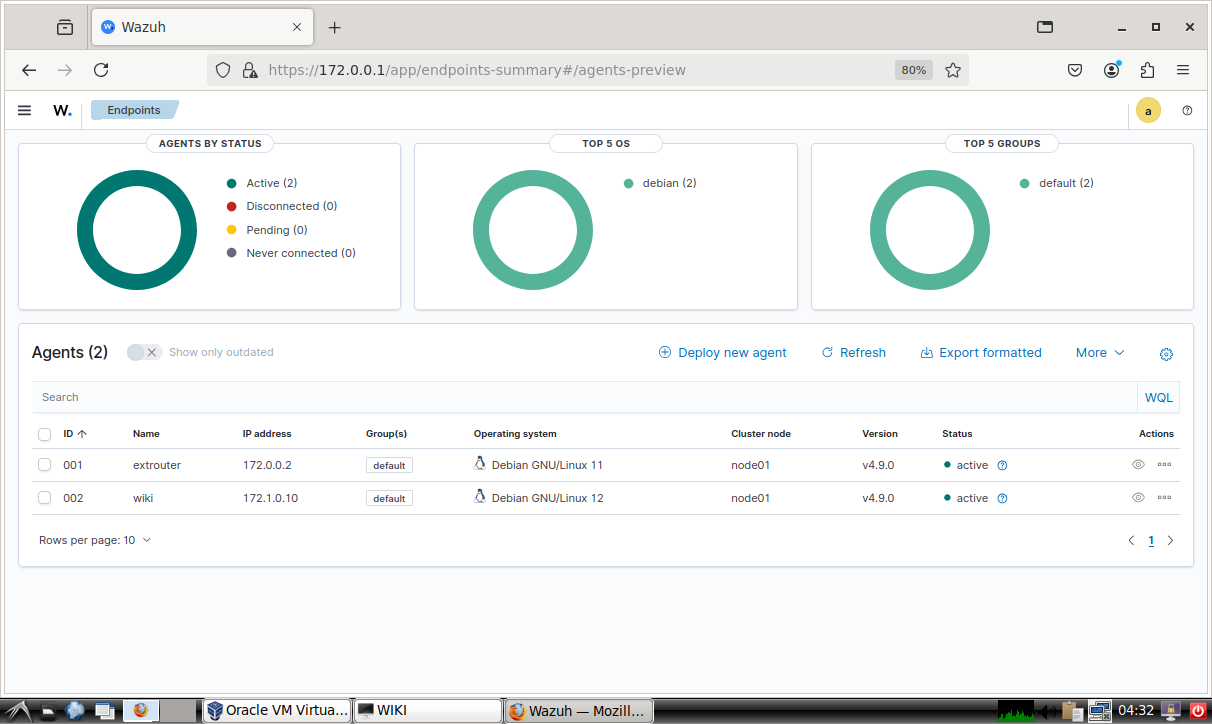
\includegraphics[width=\textwidth]{multiple active agents.png}
\caption{Multiple active agents in Wazuh (Extrouter, Wiki)}
\end{figure}

\subsection{Enhancing network security with threat intelligence}

\paragraph{Threat Intelligence and Its Role in Network Security}

Threat intelligence refers to the collection, analysis, and sharing of information about potential or existing threats that can target an organization’s network. It helps security teams stay ahead of emerging threats by providing insights into attack vectors, malicious actors, and indicators of compromise (IOCs). This information enables proactive threat detection, mitigation, and incident response to protect the network.

\paragraph{MITRE ATT\&CK Framework and Its Role in Threat Intelligence}

MITRE ATT\&CK is a globally accessible, structured framework that catalogs adversary tactics, techniques, and procedures (TTPs) used by attackers across different phases of a cyberattack. It serves as a valuable threat intelligence source by detailing how attackers operate and what actions they take to compromise systems.

\begin{description}
	\item[Detection] SIEM tools like Wazuh can map incoming alerts to specific techniques described in the MITRE ATT\&CK framework. This helps detect threats more accurately by identifying known behaviors such as credential dumping or phishing attacks.
	
	\item[Classification] Security events can be classified into phases (e.g., initial access, lateral movement, privilege escalation) based on MITRE ATT\&CK’s catalog. This structured classification assists in understanding where the attack stands in the kill chain and helps prioritize responses.
	
	\item[Mitigation]The framework provides actionable advice on countermeasures for each tactic and technique, helping organizations build effective defensive strategies. SIEM platforms can use this intelligence to automate threat responses or recommend specific actions to mitigate detected attacks.
	
\end{description}

\subsection{Identifying network attack techniques with MITRE ATT\&CK}

\paragraph{Adversary Groups Using Password Spraying}
\begin{description}
	\item[Silent Librarian (G0122)] This group targets universities, research institutes, and government agencies to steal academic data and intellectual property. They are known to have affiliations with the Iranian government, using cyber intrusions to gather sensitive information.
	
	\item[Leafminer (G0077)] An Iranian threat group targeting government and business entities in the Middle East. They focus on exploiting vulnerabilities for espionage and persistent access to compromised systems.
	
	\item[Lazarus Group (G0032)] A North Korean state-sponsored group linked to financial theft and destructive cyber campaigns, including major breaches like the Sony Pictures attack. They use credential-based attacks, including password spraying, to achieve access and conduct espionage or financial gain.

\end{description}

\paragraph{Mitigation Strategies for Password Spraying}
\begin{description}
	\item[Password Policies (M1027)] Implementing strict password complexity policies to reduce the use of common passwords that can be easily guessed by attackers. This includes enforcing a minimum length and combination of characters.
	
	\item[Multi-Factor Authentication (MFA) (M1032)] Adding an additional layer of security, such as one-time passwords (OTPs) or hardware tokens, ensures that compromised credentials alone are not sufficient for access.
	
	\item[Account Use Policies (M1036)] Limiting the number of login attempts and implementing account lockouts after multiple failed attempts can prevent password spraying attacks from succeeding.
\end{description}

\paragraph{Software Tools Used in Password Spraying Attacks}
\begin{description}
	\item[MailSniper (S0413)] A penetration testing tool often used to search for credentials and sensitive information in Microsoft Exchange environments. It can automate password spraying against email systems to compromise accounts.
	
	\item[Bad Rabbit (S0606)] A self-propagating ransomware that relies on credential access techniques, including password spraying, to spread across networks and systems rapidly. It is associated with attacks on transportation sectors and organizations in Eastern Europe and Russia.
\end{description}

\begin{figure}[H]
\centering
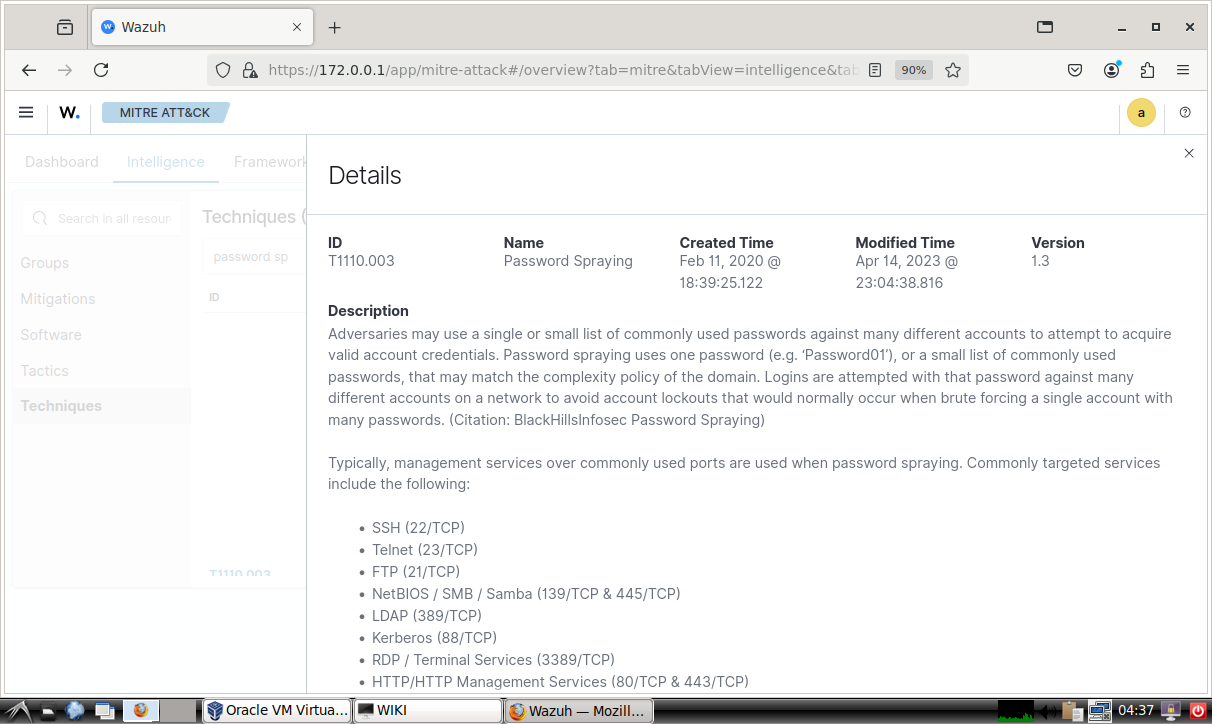
\includegraphics[width=\textwidth]{ATTK 1 PIC 1.png}
\caption{MITRE ATT\&CK 1 Part 1}
\end{figure}
\begin{figure}[H]
\centering
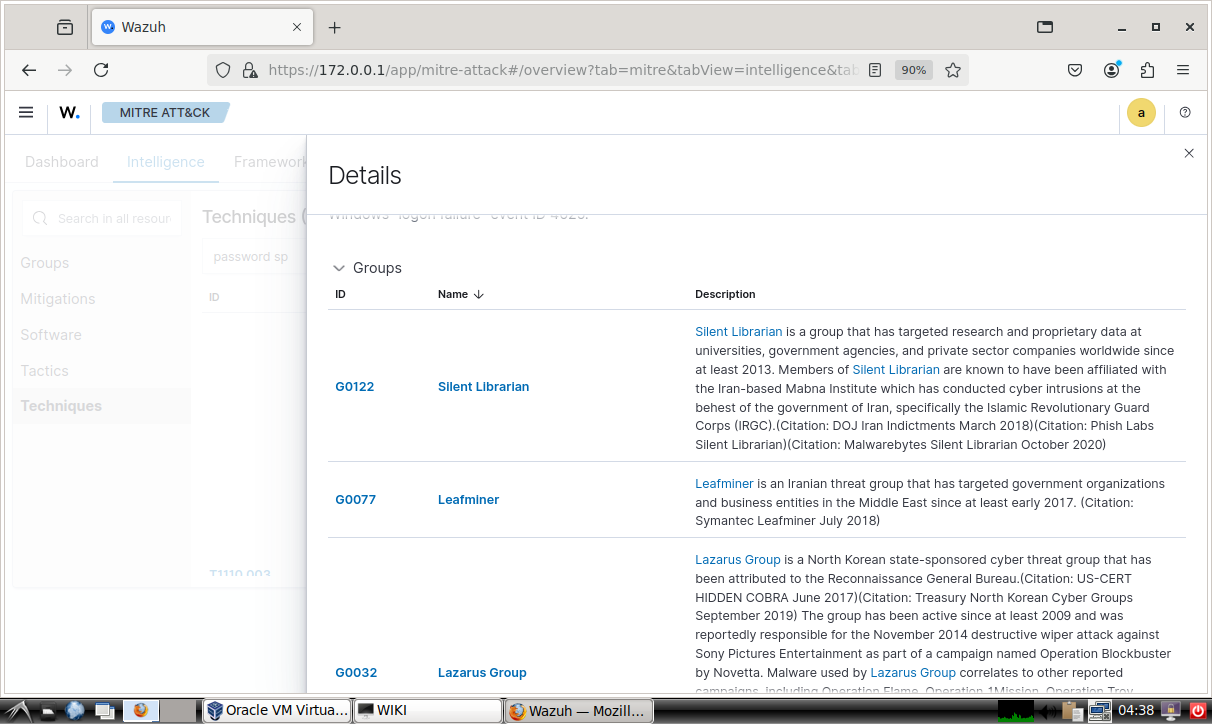
\includegraphics[width=\textwidth]{ATTK 1 PIC 2.png}
\caption{MITRE ATT\&CK 1 Part 2}
\end{figure}
\begin{figure}[H]
\centering
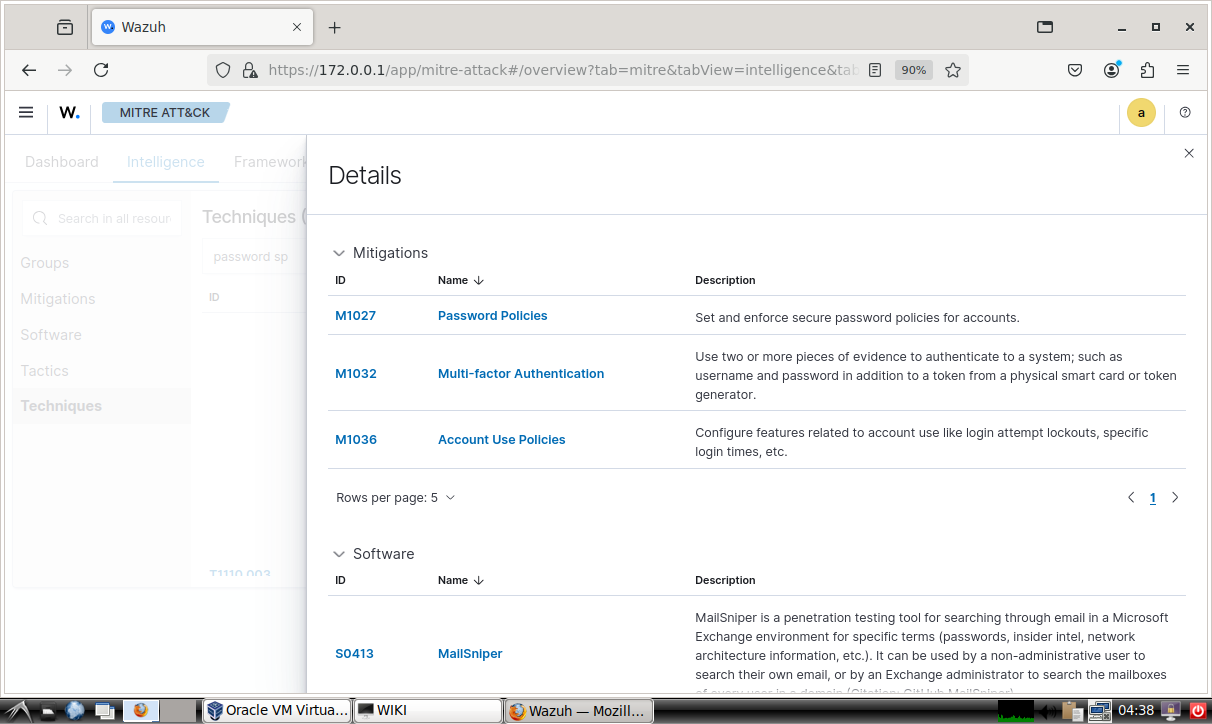
\includegraphics[width=\textwidth]{ATTK 1 PIC 3.png}
\caption{MITRE ATT\&CK 1 Part 3}
\end{figure}
\begin{figure}[H]
\centering
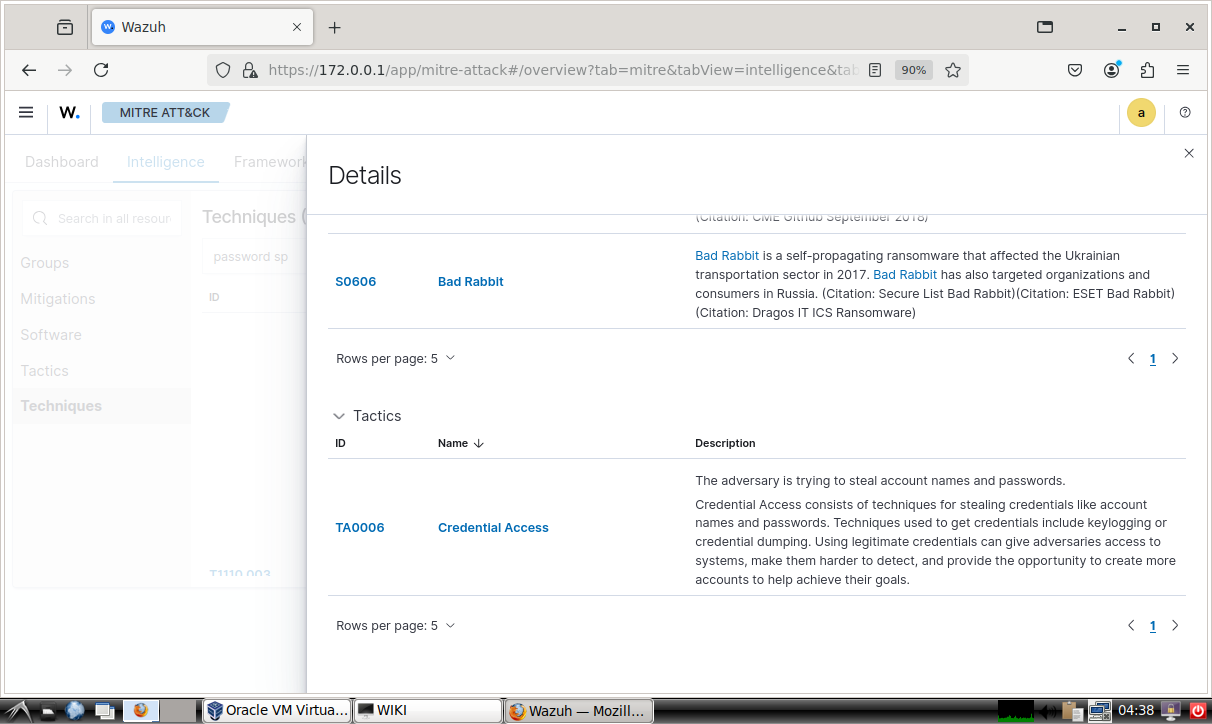
\includegraphics[width=\textwidth]{ATTK 1 PIC 4.png}
\caption{MITRE ATT\&CK 1 Part 4}
\end{figure}

\newpage

\paragraph{Adversary Groups Using Authentication Package}
\begin{description}
	\item[No specific adversary groups] There are no specific adversary groups explicitly identified associated with this technique (T1547.002 – Authentication Package). However, this attack vector is used for persistence and privilege escalation, typically by sophisticated groups looking to maintain access in compromised systems.
\end{description}

\paragraph{Mitigation Strategies For Authentication Package}
\begin{description}
	\item[Privileged Process Integrity (M1025)] Protecting processes with high privileges through mechanisms such as protected process light (PPL), anti-injection defenses, and strict enforcement of process integrity policies. This helps ensure that only trusted binaries can run with elevated privileges, reducing the risk of malicious DLLs being loaded.
	
	\item[Registry Monitoring] Regular monitoring of Windows registry keys, especially the HKLM/ SYSTEM/ CurrentControlSet/ Control/ Lsa key, can detect unauthorized changes used to load malicious authentication packages. Alerting on suspicious modifications can help in detecting an active attack early.
	
	\item[Application Whitelisting] Implementing application whitelisting ensures that only trusted executables can run on the system. This makes it harder for attackers to introduce malicious DLLs into the Local Security Authority (LSA) process for persistence.
\end{description}

\paragraph{Software Tools Used in Authentication Package Attack}
\begin{description}
	\item[Flame (S0143)] Flame is a sophisticated malware toolkit known for collecting information from systems, primarily targeting entities in the Middle East. It exploits various techniques, including privilege escalation, to gain and maintain persistence on the victim’s machine. Flame can leverage techniques such as the authentication package attack to execute code during system startup and maintain long-term access.
\end{description}

\begin{figure}[H]
\centering
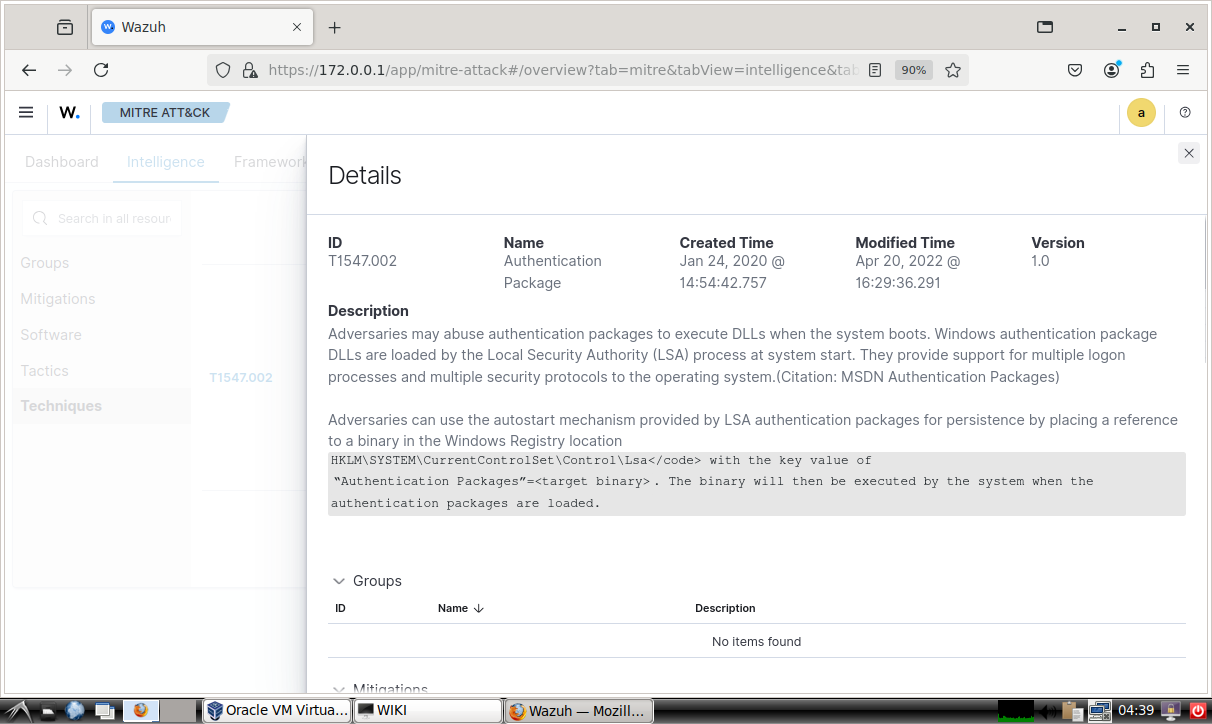
\includegraphics[width=\textwidth]{ATTK 2 PIC 01.png}
\caption{MITRE ATT\&CK 2 Part 1}
\end{figure}

\begin{figure}[H]
\centering
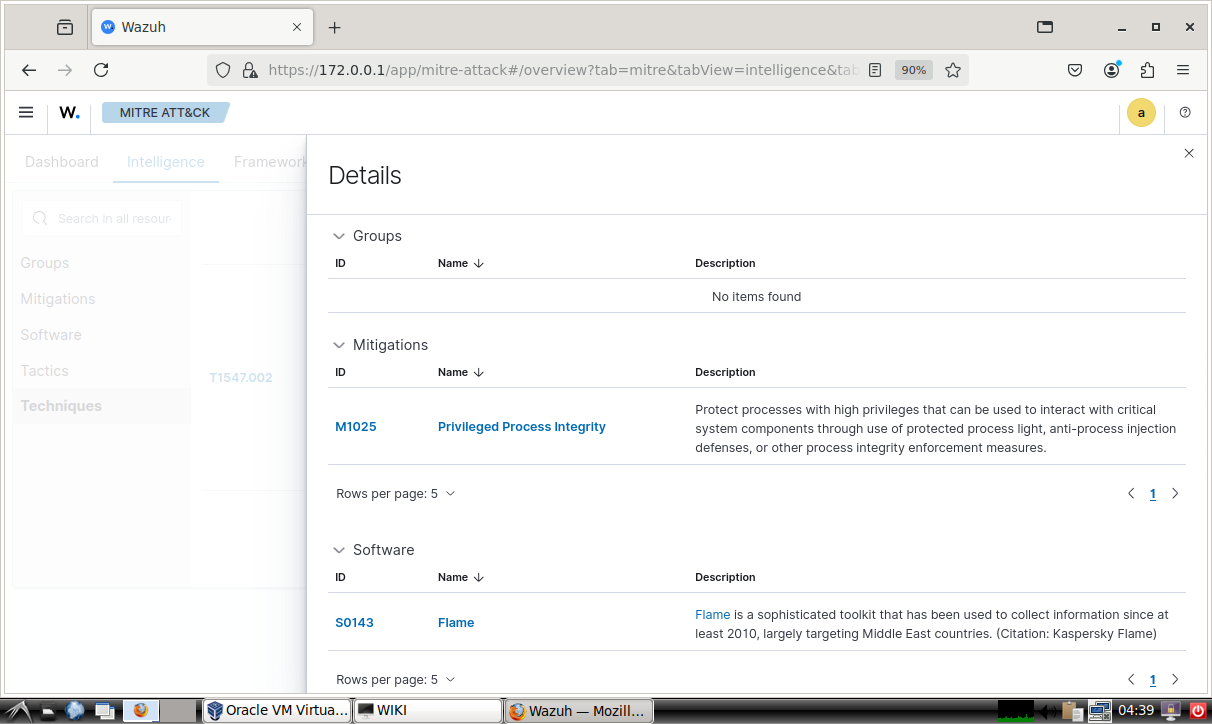
\includegraphics[width=\textwidth]{ATTK 2 PIC 02.png}
\caption{MITRE ATT\&CK 2 Part 2}
\end{figure}

\begin{figure}[H]
\centering
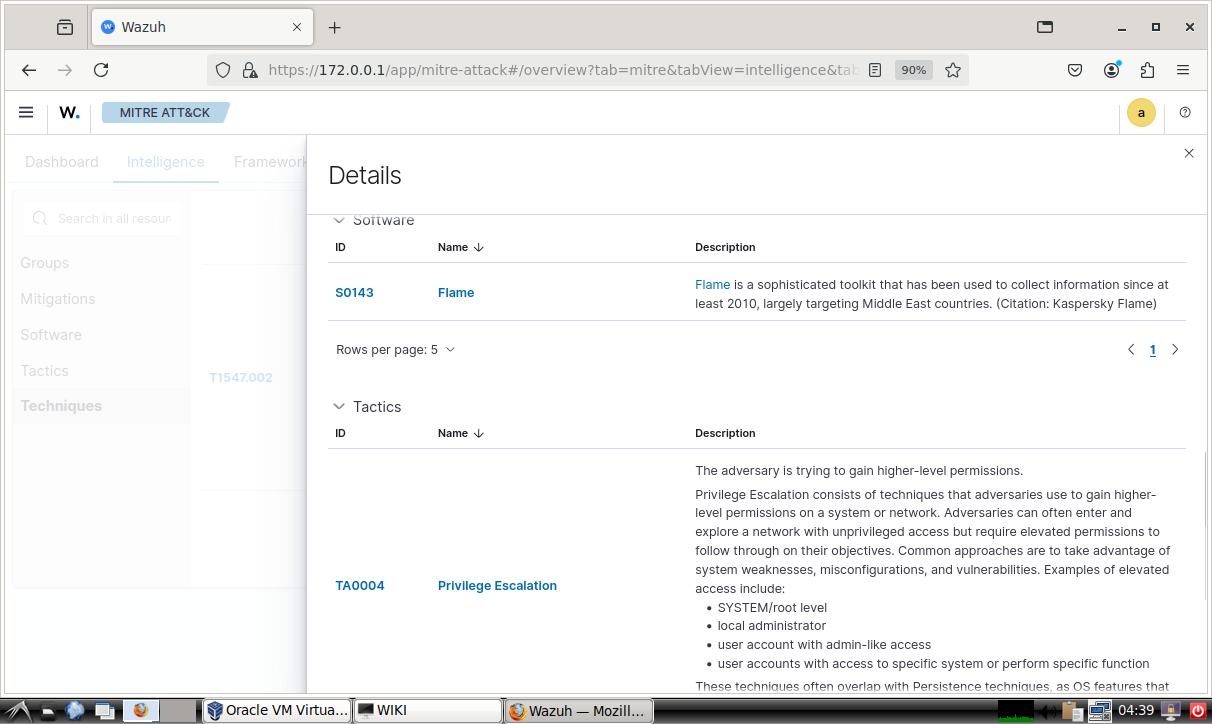
\includegraphics[width=\textwidth]{ATTK 2 PIC 03.png}
\caption{MITRE ATT\&CK 2 Part 3}
\end{figure}

\subsection{Complementary Control to SIEM and Threat Intel}
A complementary control to SIEM and threat intelligence is Endpoint Detection and Response (EDR), which provides real-time monitoring and threat detection at the endpoint level. While SIEM aggregates and correlates logs from across the network, EDR focuses on identifying suspicious behavior on individual devices, such as malware infections or unauthorized access attempts. EDR integrates with SIEM by feeding detailed endpoint data and alerts, enhancing visibility and enabling faster incident response. Additionally, EDR leverages threat intelligence to detect known indicators of compromise (IOCs) and can automatically contain threats by isolating compromised endpoints, creating a more comprehensive security framework. Together, SIEM, EDR, and threat intelligence ensure robust, multi-layered protection across both networks and endpoints.


\end{document}